%==============================================================================
%  An Energy-Aware Extension of Raft with Observer Roles and Provisional
%  Consensus for IoT
%
%  IEEE conference format (IEEEtran).
%  Compile with any of:
%      pdflatex main && pdflatex main
%      tectonic -X compile main.tex
%
%  Figures that are pre-generated images:
%      figures/energy.png              (from ../results/energy.png)
%      figures/latency_messages.png    (from ../results/latency_messages.png)
%      figures/availability.png        (from ../results/availability.png)
%      figures/dashboard.png           (OPTIONAL: screenshot of the Flask
%                                       dashboard; the figure env is currently
%                                       commented out in Section IV).
%==============================================================================

\documentclass[conference]{IEEEtran}
\IEEEoverridecommandlockouts

\usepackage{cite}
\usepackage{amsmath,amssymb,amsfonts}
\usepackage{float}
\usepackage{algorithm}
\usepackage{algorithmic}
\usepackage{graphicx}
\usepackage{textcomp}
\usepackage{xcolor}
\usepackage{booktabs}
\usepackage{url}
\usepackage[hidelinks]{hyperref}
\usepackage{tikz}
\usetikzlibrary{arrows.meta,positioning,shapes.geometric,fit,calc,backgrounds}
\usepackage{listings}
\usepackage{xspace}

% Compact code listing style.
\lstset{
  basicstyle=\ttfamily\footnotesize,
  breaklines=true,
  columns=fullflexible,
  frame=single,
  xleftmargin=2pt,
  xrightmargin=2pt,
}

% Protocol-name shortcuts.  Renamed to avoid clashing with any TeX primitive.
\newcommand{\echoproto}{\textsc{Echo}\xspace}
\newcommand{\raftproto}{\textsc{Raft}\xspace}
\newcommand{\echodproto}{\textsc{echoD}\xspace}

\def\BibTeX{{\rm B\kern-.05em{\sc i\kern-.025em b}\kern-.08em
    T\kern-.1667em\lower.7ex\hbox{E}\kern-.125emX}}

\begin{document}

\title{An Energy-Aware Extension of Raft with Observer Roles
  and Provisional Consensus for IoT Clusters}

\author{
  \IEEEauthorblockN{Ashwanth Kumaravel \quad Sreenandu G}
  \IEEEauthorblockA{Vellore Institute of Technology, Chennai, India\\
                    Email: ashwanth.kumaravel2023@vitstudent.ac.in,\;
                    sreenandu.g2023@vitstudent.ac.in}
}

\maketitle

%------------------------------------------------------------------------------
\begin{abstract}
Raft~\cite{ongaro2014raft} is widely used for replication in distributed
systems, but its assumptions of homogeneous, always-powered participants
and periodic heartbeats are expensive in battery-powered IoT clusters.
Recent work has extended Raft along three broad axes: \emph{energy-aware
operation} (EDRaft~\cite{barros2023edraft}, Energy-Efficient
Raft~\cite{nakagawa2017energy}, Weighted RAFT~\cite{xu2021weighted}),
\emph{lightweight or witness-style participants}~\cite{paris2015reducing,
blanco2023pycloudiot}, and \emph{hierarchical or adaptive leader selection}
(LH-Raft~\cite{guo2022lhraft}, MCRaft~\cite{xu2022mcraft},
DQN-Raft~\cite{liu2022dqnraft}, LRD-Raft~\cite{yang2025lrdraft}). We
present \echoproto, a crash-fault-tolerant variant of Raft that unifies
three of these ideas into a single protocol: (i)~an \emph{observer} role
for coordinators whose battery drops below a configurable threshold,
with hysteretic re-entry; (ii)~an \emph{event-driven consensus trigger}
mechanism that replaces periodic full \texttt{AppendEntries} heartbeats
with $\sim$32-byte liveness pings plus on-demand replication rounds;
and (iii)~\emph{provisional consensus}, a partition-tolerance mechanism
that lets sub-clusters make local progress under a distinct partition
epoch and reconciles on heal while preserving Raft's safety properties
on the globally-committed prefix. Measuring \echoproto\ against
\raftproto\ under an identical, matched sensor workload--fixing an
asymmetry present in an earlier version of this harness--exposed
\echoproto's own inefficiencies: a liveness ping broadcast to every
node accounts for 75--80\% of its total traffic, and unweighted random
election timeouts repeatedly split votes. We therefore present a second
protocol, \echodproto, a Raft/\echoproto\ hybrid that keeps
\echoproto's tiered topology and provisional consensus but adds six
targeted optimizations--edge-side delta filtering, batched
event-driven consensus, coordinators-only adaptive liveness,
battery-ordered election timeouts, directed leader handoff, and
batched partition reconciliation--none of which weakens \raftproto's
safety argument. On a matched 5-coordinator, 10-leaf, 5-second workload,
\echodproto\ uses $4$--$6\times$ fewer messages than \raftproto\ and
\echoproto\ while keeping commit latency and cluster availability equal
or better. We implement all three protocols on a shared asyncio message
bus ($\approx$4~KLOC Python) and release a hardware-free MQTT system
that runs any of the three over real network transport, with a
Flask+Socket.IO dashboard. The codebase is open source.
\end{abstract}

\begin{IEEEkeywords}
distributed consensus, Raft, Internet of Things, energy-aware protocols,
network partitions, MQTT, edge computing.
\end{IEEEkeywords}

%==============================================================================
\section{Introduction}
%==============================================================================

The steady growth of Internet-of-Things (IoT) deployments has intensified
the need for consensus algorithms that are robust to the particular
constraints of edge environments: limited device power, intermittent
wireless connectivity, and heterogeneous node capabilities. \raftproto\
\cite{ongaro2014raft,ongaro2014dissertation} has become the default
consensus building block for many IoT and blockchain systems because it
is simpler to understand and implement than Paxos~\cite{lamport1998paxos}
while providing equivalent safety guarantees.

Standard \raftproto\ is not, however, optimised for energy efficiency or
for the dynamic role adaptation that IoT clusters demand
\cite{barros2023edraft,paris2015reducing,howard2021arc}. Three concrete
pain points recur:

\begin{enumerate}
\item \emph{Low-battery nodes remain full voters until they fail.} A
  coordinator near depletion can still be elected leader and then die
  mid-term, forcing re-elections that further drain healthy peers
  \cite{barros2023edraft,nakagawa2017energy}.
\item \emph{Idle traffic is dominated by heartbeats.} Empty
  \texttt{AppendEntries} RPCs every 50--150~ms dominate per-node transmit
  energy in duty-cycled deployments, even when nothing needs to be
  replicated \cite{paris2015reducing,xu2021weighted}.
\item \emph{Strict partition liveness is undesirable.} Many IoT
  applications--local telemetry, rate-limited actuation--prefer bounded
  local progress with deferred reconciliation over blocking all writes
  until the network heals \cite{blanco2023pycloudiot,yang2025lrdraft}.
\end{enumerate}

\paragraph*{Contributions} This paper presents \echoproto, an extension
of \raftproto\ targeting energy-constrained clusters. Concretely:

\begin{itemize}
\item A battery-aware \textbf{observer role} with hysteretic re-entry
  ($T_{\text{low}}{=}15\%$, $T_{\text{restore}}{=}25\%$), an energy-gated
  vote predicate, and an energy-weighted election tiebreaker. This draws
  on the witness/observer idea of Pâris and Long~\cite{paris2015reducing}
  and the layered node classification of
  PyCloudIoT~\cite{blanco2023pycloudiot}, but integrates it into the Raft
  election path directly rather than as a separate tier.
\item \textbf{Event-driven replication triggers}. Full
  \texttt{AppendEntries} traffic is replaced with $\sim$32-byte liveness
  pings, and real replication only fires on typed triggers (\texttt{Delta},
  \texttt{Join}, \texttt{Partition}, \texttt{Reconcile},
  \texttt{Liveness}). This is a natural generalisation of the
  message-reduction goals of EDRaft~\cite{barros2023edraft} and
  Energy-Efficient Raft~\cite{nakagawa2017energy}.
\item \textbf{Provisional consensus}. A partition-epoch field in
  \texttt{AppendEntries} allows sub-clusters to replicate locally under
  partition; a deterministic reconciliation procedure truncates losing-side
  provisional entries and re-proposes them as new commands on heal,
  preserving the Raft safety argument on the reconciled committed prefix.
\item \echodproto, \textbf{a Raft/\echoproto\ hybrid} that keeps
  \echoproto's tiered topology, energy gating, and provisional
  consensus, and adds six efficiency optimizations--edge-side delta
  filtering, batched event-driven consensus, coordinators-only adaptive
  liveness, battery-ordered election timeouts, directed leader handoff,
  and batched partition reconciliation--motivated directly by measuring
  where \echoproto's own traffic was wasted.
\item A \textbf{shared implementation} of \raftproto, \echoproto, and
  \echodproto\ over a common asyncio message bus for like-for-like
  measurement, plus a hardware-free MQTT system that runs any of the
  three protocols over real network transport, with a Flask+Socket.IO
  dashboard.
\item An \textbf{empirical methodology} with an identical, seeded
  workload replayed across all three protocols, plus an experiment
  harness that reproduces the same metrics over real MQTT transport for
  future hardware validation.
\end{itemize}

The paper is organised as follows. Section~\ref{sec:background} reviews
\raftproto\ and summarises the literature on energy-aware, witness-based,
hierarchical, and reinforcement-learning-based Raft variants.
Section~\ref{sec:design} details the \echoproto\ protocol.
Section~\ref{sec:echod} presents \echodproto, the six optimizations it
adds on top of \echoproto, and its positioning relative to prior art.
Section~\ref{sec:impl} describes the implementation.
Section~\ref{sec:safety} sketches the safety argument.
Section~\ref{sec:eval} presents the evaluation methodology and
matched-workload results for all three protocols.
Sections~\ref{sec:discussion}--\ref{sec:conclusion} discuss limitations,
open questions, and next steps.

%==============================================================================
\section{Background and Related Work}\label{sec:background}
%==============================================================================

\subsection{Raft in one paragraph}
\raftproto~\cite{ongaro2014raft} elects a single leader per
monotonically increasing term using randomised election timeouts. The
leader replicates log entries via \texttt{AppendEntries} RPCs; an entry
is committed once a majority of servers has persisted it. Safety rests
on five properties--election safety, leader append-only, log matching,
leader completeness, and state-machine safety. Howard's ARC
thesis~\cite{howard2021arc} gives a formal treatment of these properties
and is the reference used throughout this paper.

\subsection{Energy-aware Raft variants}
EDRaft~\cite{barros2023edraft} reframes leader selection as a
\emph{collective} decision that prioritises group uptime over individual
optimality; the authors report leader uptime up to 70\% longer than
standard \raftproto\ under extended low-power runs. Nakagawa and
Hayashibara's Energy-Efficient Raft~\cite{nakagawa2017energy} reduces
the message count per round by coalescing control traffic and duty-cycling
non-leader nodes. Weighted RAFT~\cite{xu2021weighted} assigns per-node
weights that reflect compute or network cost and uses them to bias the
election, reducing unnecessary leader churn in heterogeneous IoT
blockchains. \echoproto's contribution here is the \emph{observer role}:
rather than weighting votes, low-energy nodes leave the voting set
entirely, and re-enter only after a hysteresis gap.

\subsection{Witness and lightweight-participant roles}
Pâris and Long~\cite{paris2015reducing} were among the first to show
that replacing some full replicas with \emph{witnesses}--nodes that
vote but do not store state--reduces the energy footprint of a
distributed consensus cluster while preserving fault tolerance.
PyCloudIoT~\cite{blanco2023pycloudiot} extends this to an
energy-efficient FaaS edge platform that classifies nodes by energetic
and computational capability and orchestrates them accordingly. Our
observer role is compatible with both of these ideas but is dynamic:
a coordinator that begins as a full voter can become an observer
mid-deployment when its battery drops, and can rejoin later.

\subsection{Hierarchical and adaptive models}
LH-Raft~\cite{guo2022lhraft} forms location- or reputation-based
candidate groups so that leader elections are localised before global
agreement is reached; this reduces communication overhead in large
IoT-blockchain deployments. MCRaft~\cite{xu2022mcraft} distributes
leadership among multiple super-nodes to improve cluster stability.
Zuo \emph{et al.}~\cite{zuo2024raftgrouping} group Raft peers using
affinity-propagation clustering to reduce inter-group traffic. Our
tiered topology (coordinators + leaves) is compatible with these
designs: leaves could be clustered under a subset of coordinators along
LH-Raft lines, which we leave as future work.

\subsection{Reinforcement-learning-based leader selection}
DQN-Raft~\cite{liu2022dqnraft} and its successor
DQN-Raft+~\cite{wang2025dqnraftplus} use deep Q-learning to choose
leaders based on observed reward signals, improving adaptability on
heterogeneous networks. LRD-Raft~\cite{yang2025lrdraft} decouples log
replication from leader traffic to balance load and improve energy
efficiency in consortium-blockchain IoT. These techniques are
orthogonal to \echoproto's contributions; a ``DQN-\echoproto'' that
learns when to lower $T_{\text{low}}$ dynamically is a natural future
direction. Hybrid Raft--PoW designs~\cite{ulukok2025hybridraftpow} take
yet another angle by composing Raft with a proof-of-work layer for
tamper resistance.

\subsection{Partition-tolerant consensus}
Classical \raftproto\ and systems built on it tolerate partitions by
blocking progress on the minority side. Eventual-consistency stores
allow partition writes at the cost of weaker semantics. Variants such
as Flexible Paxos~\cite{howard2016flexible} and
EPaxos~\cite{moraru2013epaxos} tune quorum \emph{shape} for latency or
locality but do not introduce explicit provisional writes. \echoproto\
occupies the intermediate design point: provisional entries are never
globally committed, so reads over the committed prefix remain
linearisable, but each sub-cluster can durably accumulate locally
ordered proposals that are re-proposed after heal.

\subsection{Energy-aware routing at the same layer}
Outside the consensus literature, a large body of work on energy-aware
routing in IoT and wireless sensor networks informs the constants used
in this paper: Shah \emph{et al.}'s throughput-optimised clustered
routing~\cite{shah2018energy}, Samadi \emph{et al.}'s SDN-based
intelligent energy-aware routing~\cite{samadi2023intelligent}, and
Kang and Jeon's UAV-enabled aggregation~\cite{kang2024uav}. These
provide useful priors for realistic drain rates; they do not change the
protocol but they do constrain the experiment design.

%==============================================================================
\section{ECHO Protocol Design}\label{sec:design}
%==============================================================================

\subsection{Topology and node roles}
An \echoproto\ cluster is organised in two tiers
(Fig.~\ref{fig:topology}):
\begin{itemize}
\item \textbf{Coordinators} run the consensus state machine and
  replicate a log. A typical deployment uses 3--7 coordinators.
\item \textbf{Leaves} are lightweight sensor sources. They register
  with a coordinator and forward \texttt{SensorDataReport} messages;
  they do not participate in voting.
\end{itemize}

\begin{figure}[t]
\centering
\resizebox{\columnwidth}{!}{%
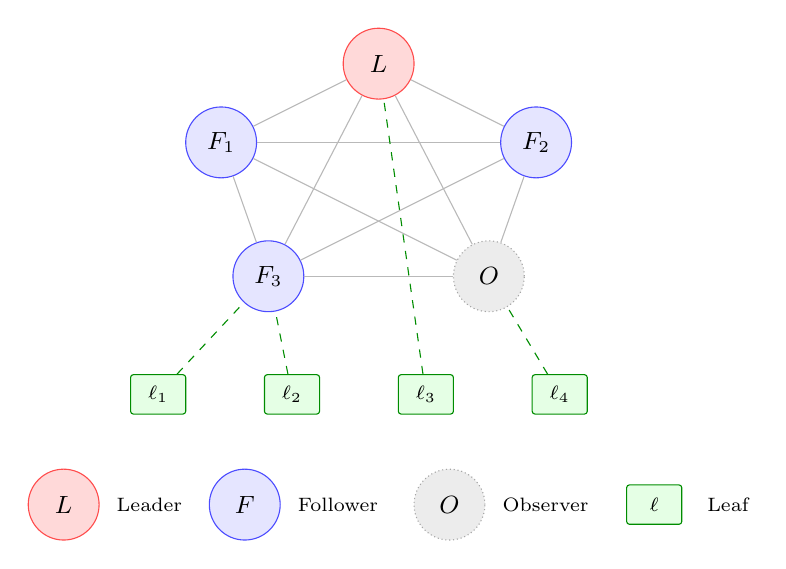
\begin{tikzpicture}[
    every node/.style={font=\footnotesize},
    leader/.style   ={circle,draw=red!70,fill=red!15,
                     minimum size=9mm,inner sep=0pt,font=\bfseries\small},
    follower/.style ={circle,draw=blue!70,fill=blue!10,
                     minimum size=9mm,inner sep=0pt,font=\small},
    observer/.style ={circle,draw=gray!70,fill=gray!15,
                     minimum size=9mm,inner sep=0pt,
                     densely dotted,font=\small},
    leafnode/.style ={rectangle,rounded corners=1pt,
                     draw=green!55!black,fill=green!10,
                     minimum width=7mm,minimum height=5mm,
                     inner sep=1pt,font=\scriptsize},
    mesh/.style     ={-,gray!55,thin},
    leafedge/.style ={-,green!55!black,dashed,thin},
  ]
  % --- coordinators (pentagon-ish layout) ---
  \node[leader]   (L)  at ( 0.0, 1.7) {$L$};
  \node[follower] (F1) at (-2.0, 0.7) {$F_1$};
  \node[follower] (F2) at ( 2.0, 0.7) {$F_2$};
  \node[follower] (F3) at (-1.4,-1.0) {$F_3$};
  \node[observer] (O)  at ( 1.4,-1.0) {$O$};

  % full mesh
  \draw[mesh] (L)--(F1);  \draw[mesh] (L)--(F2);
  \draw[mesh] (L)--(F3);  \draw[mesh] (L)--(O);
  \draw[mesh] (F1)--(F2); \draw[mesh] (F1)--(F3);
  \draw[mesh] (F1)--(O);  \draw[mesh] (F2)--(F3);
  \draw[mesh] (F2)--(O);  \draw[mesh] (F3)--(O);

  % --- leaves below ---
  \node[leafnode] (l1) at (-2.8,-2.5) {$\ell_1$};
  \node[leafnode] (l2) at (-1.1,-2.5) {$\ell_2$};
  \node[leafnode] (l3) at ( 0.6,-2.5) {$\ell_3$};
  \node[leafnode] (l4) at ( 2.3,-2.5) {$\ell_4$};
  \draw[leafedge] (l1) -- (F3);
  \draw[leafedge] (l2) -- (F3);
  \draw[leafedge] (l3) -- (L);
  \draw[leafedge] (l4) -- (O);

  % --- legend as a compact row at bottom ---
  \begin{scope}[shift={(-4.0,-3.9)},
                every node/.style={font=\scriptsize}]
     \node[leader]     (gL) at (0.0,0) {$L$};
     \node[anchor=west]      at (0.55,0) {Leader};
     \node[follower]   (gF) at (2.3,0) {$F$};
     \node[anchor=west]      at (2.85,0) {Follower};
     \node[observer]   (gO) at (4.9,0) {$O$};
     \node[anchor=west]      at (5.45,0) {Observer};
     \node[leafnode]   (gl) at (7.5,0) {$\ell$};
     \node[anchor=west]      at (8.05,0) {Leaf};
  \end{scope}
\end{tikzpicture}%
}
\caption{Tiered \echoproto\ cluster. Coordinators ($L$, $F_i$, $O$) form
a full mesh and run consensus; leaves $\ell_i$ register with a coordinator
and only send sensor reports. An observer is a coordinator whose battery
has dropped below $T_{\text{low}}$; it has left the voting quorum but
still receives log updates.}
\label{fig:topology}
\end{figure}

\subsection{States and energy gating}
A coordinator's state space extends \raftproto\ with two additional
states (Fig.~\ref{fig:states}):
\begin{itemize}
\item \textbf{Observer}--entered from any non-observer state when
  $\text{battery} < T_{\text{low}}$ (default 15\%). An observer does
  not vote, is not counted toward the active quorum, and cannot
  transition to candidate. It still receives \texttt{AppendEntries} and
  keeps its log current. It re-enters as \textbf{Follower} when
  $\text{battery} \ge T_{\text{restore}}$ (default 25\%). The hysteresis
  gap prevents oscillation.
\item \textbf{Local leader}--a coordinator that was leader when a
  partition was detected. It continues to replicate within its
  sub-cluster under a non-zero partition epoch and rejoins as follower
  after reconciliation.
\end{itemize}

\begin{figure}[t]
\centering
\resizebox{\columnwidth}{!}{%
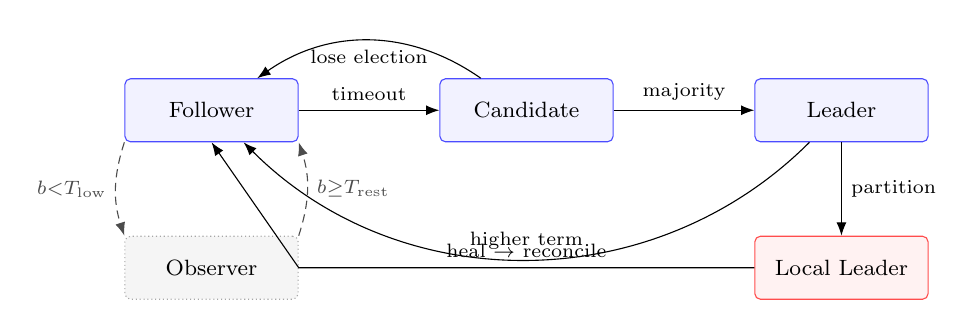
\begin{tikzpicture}[
    node distance=12mm and 22mm,
    every node/.style={font=\footnotesize},
    st/.style   ={rectangle,rounded corners=2pt,draw=blue!70,
                  fill=blue!5,minimum width=22mm,minimum height=8mm,
                  align=center},
    obs/.style  ={rectangle,rounded corners=2pt,draw=gray!70,
                  densely dotted,fill=gray!8,minimum width=22mm,
                  minimum height=8mm,align=center},
    lldr/.style ={rectangle,rounded corners=2pt,draw=red!70,
                  fill=red!5,minimum width=22mm,minimum height=8mm,
                  align=center},
    >=Latex, thin,
    trans/.style       ={->,thin},
    energyedge/.style  ={->,thin,densely dashed,gray!60!black},
  ]
  % Top row: normal Raft cycle
  \node[st]  (F) at (0,2.0) {Follower};
  \node[st]  (C) at (4,2.0) {Candidate};
  \node[st]  (L) at (8,2.0) {Leader};

  % Bottom row: ECHO additions
  \node[obs]  (O)  at (0,0) {Observer};
  \node[lldr] (LL) at (8,0) {Local Leader};

  % Normal Raft transitions
  \draw[trans] (F) -- node[above,font=\scriptsize]{timeout}   (C);
  \draw[trans] (C) -- node[above,font=\scriptsize]{majority}  (L);
  \draw[trans] (C) to[bend right=35]
        node[below,font=\scriptsize,pos=0.5]{lose election}    (F);
  \draw[trans] (L) to[bend left=45]
        node[above,font=\scriptsize,pos=0.5]{higher term}      (F);

  % Energy gate (dashed) - Follower <-> Observer
  \draw[energyedge] (F.south west) to[bend right=18]
        node[left,font=\scriptsize]{$b{<}T_{\text{low}}$}      (O.north west);
  \draw[energyedge] (O.north east) to[bend right=18]
        node[right,font=\scriptsize]{$b{\geq}T_{\text{rest}}$} (F.south east);

  % Partition: Leader <-> LocalLeader
  \draw[trans] (L) -- node[right,font=\scriptsize]{partition}  (LL);
  \draw[trans] (LL.west) to[bend left=0]
        node[above,font=\scriptsize,pos=0.5]{heal $\to$ reconcile}
        (F |- LL.west -| F.south east) -- ++(0,0) -- (F.south);
\end{tikzpicture}%
}
\caption{Coordinator state machine. Solid arrows: standard \raftproto.
Dashed arrows: \echoproto's energy gate (also applies from
Candidate/Leader, not drawn for clarity). Leader transitions to Local
Leader on partition and reconciles back to Follower on heal.}
\label{fig:states}
\end{figure}

\subsection{Energy-aware voting}
Every \texttt{RequestVote} RPC carries a \texttt{battery\_level} field
in $[0,100]$. A voter rejects the RPC if any standard \raftproto\ check
fails \emph{or} if $\text{battery\_level} < T_{\text{low}}$. In effect,
low-energy nodes cannot become leaders, and the cluster does not pay the
cost of re-electing after their foreseeable depletion.

For tie-breaking among simultaneous candidates, we use an
energy-weighted election score:
\begin{equation}
  \text{score}(C) \;=\; |\mathrm{votes}(C)| \cdot
    \frac{\text{battery}(C)}{\max_{C'}\text{battery}(C')}.
  \label{eq:score}
\end{equation}
The simple-majority rule still decides correctness;
(\ref{eq:score}) affects tiebreaks only. This is an important detail
for the safety argument (\S\ref{sec:safety}): no predicate is added to
the \emph{committed} path.

\subsection{Event-driven consensus triggers}
In classical \raftproto\ the leader emits a full \texttt{AppendEntries}
RPC every heartbeat interval, regardless of whether there is anything
to replicate. \echoproto\ replaces this with two mechanisms:
\begin{enumerate}
\item \textbf{Liveness pings} ($\approx$32 bytes on the wire) carry only
  $(\text{term},\text{leader\_id},\text{timestamp})$ and solely reset
  followers' election timers.
\item \textbf{Trigger-driven \texttt{AppendEntries}} only fires when a
  typed trigger is raised: \texttt{Delta} (sensor reading changes by
  more than $\Delta_{\text{thr}}{=}5\%$), \texttt{Join} (leaf
  registration), \texttt{Partition}, \texttt{Reconcile}, or
  \texttt{Liveness}. Followers buffer triggers that arrive while no
  leader is known; a newly-elected leader flushes the buffer
  immediately on promotion.
\end{enumerate}

\subsection{Provisional consensus and reconciliation}
Every \texttt{AppendEntriesRPC} carries a \texttt{partition\_epoch}
integer (0 in normal operation, incremented by
\texttt{enter\_provisional\_mode()} on partition). Log entries appended
under a non-zero epoch are tagged accordingly.

Fig.~\ref{fig:partition} shows the full flow. When a coordinator
observes a non-zero \texttt{partition\_epoch} in an incoming RPC (or
detects a partition via liveness timeout), it enters provisional mode;
the former leader of the sub-cluster becomes \emph{local leader} and
continues to replicate \emph{within} the sub-cluster. Provisional
entries never count toward the global commit index (which requires
\texttt{partition\_epoch}$=0$ and a majority of the full coordinator
set).

\begin{figure}[t]
\centering
\resizebox{\columnwidth}{!}{%
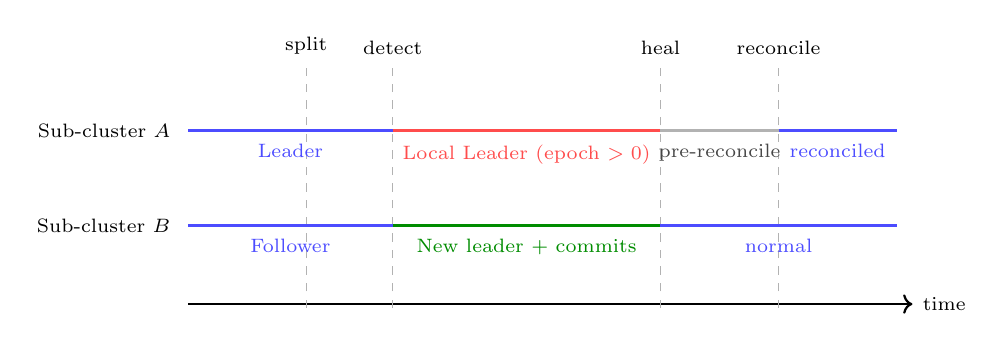
\begin{tikzpicture}[
    every node/.style={font=\scriptsize},
    evmark/.style={dashed,gray!60},
    lane/.style ={gray!50,thick},
    normal/.style={blue!70,very thick},
    prov/.style  ={red!70,very thick},
    winner/.style={green!55!black,very thick},
    wait/.style  ={gray!60,very thick},
  ]
  % time axis
  \draw[->,thick] (0,-0.2) -- (9.2,-0.2) node[right,font=\scriptsize]{time};

  % lanes (labels to the LEFT of the picture)
  \node[anchor=east,font=\scriptsize] at (-0.1,2.0) {Sub-cluster $A$};
  \node[anchor=east,font=\scriptsize] at (-0.1,0.8) {Sub-cluster $B$};
  \draw[lane] (0,2.0) -- (9,2.0);
  \draw[lane] (0,0.8) -- (9,0.8);

  % event markers (dashed vertical lines)
  \foreach \x/\lbl in {1.5/split, 2.6/detect, 6.0/heal, 7.5/reconcile} {
     \draw[evmark] (\x,-0.25) -- (\x,2.8);
     \node[above,font=\scriptsize] at (\x,2.85) {\lbl};
  }

  % Sub-cluster A segments
  \draw[normal] (0,2.0)   -- (2.6,2.0);
  \draw[prov]   (2.6,2.0) -- (6.0,2.0);
  \draw[wait]   (6.0,2.0) -- (7.5,2.0);
  \draw[normal] (7.5,2.0) -- (9.0,2.0);
  \node[below,font=\scriptsize,blue!70]        at (1.3,1.95) {Leader};
  \node[below,font=\scriptsize,red!70]         at (4.3,1.95) {Local Leader (epoch $>0$)};
  \node[below,font=\scriptsize,gray!55!black]  at (6.75,1.95){pre-reconcile};
  \node[below,font=\scriptsize,blue!70]        at (8.25,1.95){reconciled};

  % Sub-cluster B segments
  \draw[normal] (0,0.8)   -- (2.6,0.8);
  \draw[winner] (2.6,0.8) -- (6.0,0.8);
  \draw[normal] (6.0,0.8) -- (9.0,0.8);
  \node[below,font=\scriptsize,blue!70]        at (1.3,0.75){Follower};
  \node[below,font=\scriptsize,green!55!black] at (4.3,0.75){New leader + commits};
  \node[below,font=\scriptsize,blue!70]        at (7.5,0.75){normal};
\end{tikzpicture}%
}
\caption{Partition-and-heal timeline. Between \emph{detect} and
\emph{heal}, each sub-cluster progresses under its own
\texttt{partition\_epoch}. On heal, the sub-cluster with the higher
globally-committed index wins; the other truncates its provisional
entries and re-proposes them via the \texttt{Reconcile} trigger. Only
globally-committed entries ever leave the protocol.}
\label{fig:partition}
\end{figure}

On heal, the losing side--identified as the sub-cluster with the
\emph{lower} highest-globally-committed index--runs
Algorithm~\ref{alg:reconcile}:
\begin{algorithm}[H]
\small
\caption{Reconciliation on the losing sub-cluster after heal.}
\label{alg:reconcile}
\begin{algorithmic}[1]
\REQUIRE local log $L$, winning entries $E^\star$, winning commit
  index $c^\star$
\STATE $P \leftarrow \{\, e \in L : e.\text{epoch} > 0 \,\}$
  \hfill\COMMENT{provisional entries}
\IF {$c^\star > L.\text{commit\_index}$}
  \STATE truncate $L$ from index $L.\text{commit\_index}{+}1$
  \STATE append every $e \in E^\star$ to $L$
  \STATE $L.\text{commit\_index} \leftarrow c^\star$
\ENDIF
\STATE \texttt{exit\_provisional\_mode()}
\FORALL {$e \in P$}
  \STATE re-propose $(e.\text{command}, e.\text{trigger\_type})$ as
         \texttt{Reconcile} trigger
\ENDFOR
\end{algorithmic}
\end{algorithm}

Because provisional entries are never globally committed, external
observers of the replicated state machine see only entries that are
safe under \raftproto's original argument~\cite{howard2021arc};
\S\ref{sec:safety} makes this precise.

\subsection{Configuration constants}
All timing and energy parameters live in a single configuration module
so experiments are repeatable. The defaults used in this evaluation
appear in Table~\ref{tab:params}.

\begin{table}[t]
\centering
\caption{Default protocol parameters (identical across \raftproto\ and
\echoproto).}
\label{tab:params}
\setlength{\tabcolsep}{3pt}
\resizebox{\columnwidth}{!}{%
\begin{tabular}{@{}lll@{}}
\toprule
Parameter & Default & Role \\
\midrule
\texttt{ELECTION\_TIMEOUT\_MIN}   & 150\,ms  & election timer lower bound \\
\texttt{ELECTION\_TIMEOUT\_MAX}   & 300\,ms  & election timer upper bound \\
\texttt{LIVENESS\_PING\_INTERVAL} & 50\,ms   & leader keep-alive cadence \\
\texttt{PARTITION\_TIMEOUT}       & 2000\,ms & provisional entry window \\
$T_{\text{low}}$                  & 15\%     & observer entry threshold \\
$T_{\text{restore}}$              & 25\%     & observer exit threshold \\
$\Delta_{\text{thr}}$             & 5\%      & delta-trigger threshold \\
\texttt{MAX\_COORDINATORS}        & 7        & hard cluster cap \\
\texttt{SAMPLE\_INTERVAL}         & 100\,ms  & leaf polling rate \\
\bottomrule
\end{tabular}%
}
\end{table}

%==============================================================================
\section{\texorpdfstring{$\echodproto$}{echoD}: A Raft/ECHO Hybrid}\label{sec:echod}
%==============================================================================

Measuring \echoproto\ against \raftproto\ under the matched, seeded
workload described in \S\ref{sec:eval} surfaced two problems that the
original design did not anticipate. First, \echoproto's liveness ping is
broadcast to \emph{every} node--coordinators and leaves alike--every
\texttt{LIVENESS\_PING\_INTERVAL}; on a 5-coordinator, 10-leaf cluster
this single mechanism accounted for 75--80\% of \echoproto's total
message volume. Second, the energy-weighted score in
(\ref{eq:score}) only breaks ties \emph{after} an election is already
under way; because election timeouts are drawn independently and
uniformly at random, simultaneous candidacies--and the wasted
\texttt{RequestVote} rounds and re-elections they cause--were common in
practice. Neither problem is fixed by tuning \echoproto's constants;
both require moving the underlying mechanism.

\echodproto\ (``echoD'') is a second protocol that keeps \echoproto's
tiered membership, energy-gated voting, and provisional consensus
\emph{unchanged}, and adds six targeted optimizations that remove
avoidable messages without touching the vote-grant predicate or the
log-matching invariant--so the safety argument of \S\ref{sec:safety}
continues to apply verbatim (see \S\ref{sec:echod-safety}). Consensus
traffic (\texttt{RequestVote}, \texttt{AppendEntries}, liveness) never
reaches a leaf in \echodproto: leaves talk only to their own
coordinator. Table~\ref{tab:echod-compare} summarises the resulting
design points.

\begin{table}[t]
\centering
\caption{Design points across the three protocols.}
\label{tab:echod-compare}
\setlength{\tabcolsep}{2.5pt}
\footnotesize
\begin{tabular}{@{}p{13mm}p{24mm}p{24mm}p{25mm}@{}}
\toprule
 & \raftproto & \echoproto & \echodproto \\
\midrule
Topology & flat, all vote & tiered, coord.\ vote & tiered, coord.\ vote \\
Idle traffic & full \texttt{AppendEntries} to all peers & ping broadcast to \emph{all} nodes & ping to coordinators only, adaptive backoff \\
Sensor events & 1 round/event & 1 round/event, filtered post-hoc & filtered at leaf; bursts batched into 1 round \\
Elections & random timeout & random timeout, score unused & battery-ordered timeout, wins first ballot \\
Low-battery leader & dies into election gap & dies into election gap & directed handoff, no gap \\
Partition & minority halts & provisional consensus & provisional + batched reconciliation \\
\bottomrule
\end{tabular}
\end{table}

\subsection{Edge-side delta filtering}
In \echoproto, a leaf transmits every reading and the coordinator applies
the $\Delta_{\text{thr}}$ check \emph{after} the radio cost has already
been paid. \echodproto\ moves the check onto the leaf: a reading is
transmitted only if it deviates from the leaf's own last
\emph{transmitted} value by at least $\Delta_{\text{thr}}$. Sub-threshold
readings cost zero messages. The coordinator retains its own
$\Delta_{\text{thr}}$ check as a backstop for any report that reaches it
by another path (e.g.\ forwarded from a non-leader), so the mechanism is
strictly a traffic reduction, not a new source of missed events.

\subsection{Batched event-driven consensus}
Both \raftproto\ and \echoproto\ spend one consensus round per triggering
event, so a burst of $k$ simultaneous sensor readings costs $k$ rounds.
\echodproto's leader instead coalesces every trigger that arrives inside
a rolling window of \texttt{BATCH\_WINDOW\_MS} into a single log entry:
a burst of $k$ events costs one round. If the buffer reaches
\texttt{MAX\_BATCH\_SIZE} before the window closes, it flushes
immediately, so batching never adds latency under sustained load--only
under low, sparse traffic does a report wait up to
\texttt{BATCH\_WINDOW\_MS} before it is proposed.

\subsection{Coordinators-only adaptive liveness}
The leader's liveness signal is redirected to coordinators only--never
leaves--and its interval backs off geometrically while the cluster is
idle:
\begin{equation}
  I_{n+1} \;=\;
  \begin{cases}
    \texttt{LIVENESS\_PING\_INTERVAL} & \text{if consensus active since } I_n \\
    \min(I_n \cdot \beta,\; I_{\max}) & \text{otherwise,}
  \end{cases}
  \label{eq:backoff}
\end{equation}
with backoff factor $\beta{=}2$ and cap $I_{\max}{=}\texttt{ECHOD\_PING\_MAX\_INTERVAL}$,
chosen to stay below the election-timeout floor
(\S\ref{sec:echod-elections}) so backing off never triggers a spurious
election. Each coordinator separately keepalives \emph{its own} leaves
at a slow, fixed \texttt{LEAF\_KEEPALIVE\_INTERVAL}. This has a second,
unplanned benefit: in \echoproto, a leaf registered to a non-leader
coordinator was kept alive only by overhearing the leader's broadcast
ping, and would flap between \textsc{Active} and \textsc{Searching}
whenever that ping backed off or was lost; per-coordinator keepalives
remove this dependency entirely.

\subsection{Battery-ordered election timeouts}\label{sec:echod-elections}
Rather than drawing the election timeout independently of energy and
resolving ties with (\ref{eq:score}) \emph{after} an election starts,
\echodproto\ makes the timeout itself a deterministic, monotonically
decreasing function of battery:
\begin{equation}
  \tau(C) \;=\; \tau_{\min} \;+\; \bigl(1 - \text{battery}(C)\bigr)\cdot
  (\tau_{\max}-\tau_{\min}) \;+\; h(\text{id}(C)),
  \label{eq:echodtimeout}
\end{equation}
where $h(\cdot)\bmod\texttt{ELECTION\_TIE\_BREAK\_MS}$ is a stable,
deterministic per-node offset (a CRC32 hash of the node ID) that breaks
exact battery ties without introducing randomness. Because
$\tau$ is strictly decreasing in battery, the highest-battery
coordinator always reaches its deadline first, broadcasts
\texttt{RequestVote} before any other node is a candidate, and wins on
the first ballot--eliminating split votes and their wasted
\texttt{RequestVote} rounds, and selecting the energy-optimal leader as
a side effect of the timer, with no change to the vote-grant predicate
itself.

\subsection{Directed leader handoff}
When a leader's battery falls below $T_{\text{handoff}}$ (default
20\%, chosen to fire before the observer threshold $T_{\text{low}}{=}15\%$
so a leader always has time to hand off before losing its voting
rights), it nominates its highest-battery peer directly instead of
waiting to die into an election-timeout gap. Peer batteries are learned
for free from the \texttt{responder\_battery} field piggybacked on every
\texttt{AppendEntries} response. Algorithm~\ref{alg:handoff} gives the
procedure; the nominee starts an election immediately on receipt,
replacing a full randomised election ($\tau_{\min}$--$\tau_{\max}$ of
latency) with one directed message.

\begin{algorithm}[H]
\small
\caption{Directed leader handoff (leader side).}
\label{alg:handoff}
\begin{algorithmic}[1]
\REQUIRE own battery $b_0$, peer batteries $\{b_i\}$ from
  \texttt{responder\_battery}
\IF{$b_0 < T_{\text{handoff}}$ \AND handoff not yet sent this term}
  \STATE $s \leftarrow \arg\max_i b_i$ \hfill\COMMENT{ties broken by node ID}
  \IF{$b_s > b_0$}
    \STATE send \texttt{LeadershipHandoff}(term) to $s$
    \STATE step down to \textsc{Follower}; reset election timer
  \ENDIF
\ENDIF
\end{algorithmic}
\end{algorithm}

\subsection{Provisional consensus with batched reconciliation}
\echodproto\ inherits \echoproto's provisional-consensus mechanism
(\S\ref{sec:design}, Fig.~\ref{fig:partition}) unchanged: on partition,
each sub-cluster may elect a local leader and continue to replicate
under a non-zero \texttt{partition\_epoch}, and \raftproto's minority
side would simply halt in the same scenario. \echodproto's addition is
at reconciliation time only: where Algorithm~\ref{alg:reconcile} re-proposes
each truncated provisional entry as its own \texttt{Reconcile} round,
\echodproto\ re-proposes the \emph{entire} truncated suffix as a single
batch entry, so a losing sub-cluster that accumulated $m$ provisional
entries costs one round to reconcile, not $m$. Because reconciliation
happens strictly after the losing side adopts the winning side's
committed prefix (Algorithm~\ref{alg:reconcile}, lines 2--5), batching
the re-proposed commands changes only the number of rounds required,
not which entries are eligible for global commit.

\subsection{Configuration constants}
Table~\ref{tab:echod-params} lists the additional constants
\echodproto\ introduces on top of Table~\ref{tab:params} (all other
parameters are shared with \raftproto\ and \echoproto).

\begin{table}[t]
\centering
\caption{Additional \echodproto\ parameters.}
\label{tab:echod-params}
\setlength{\tabcolsep}{3pt}
\resizebox{\columnwidth}{!}{%
\begin{tabular}{@{}lll@{}}
\toprule
Parameter & Default & Role \\
\midrule
\texttt{BATCH\_WINDOW\_MS}          & 50\,ms  & consensus batching window \\
\texttt{MAX\_BATCH\_SIZE}           & 10      & immediate-flush threshold \\
\texttt{ECHOD\_PING\_MAX\_INTERVAL} & 250\,ms & adaptive ping backoff cap ($I_{\max}$) \\
\texttt{LIVENESS\_BACKOFF\_FACTOR}  & 2.0     & backoff rate ($\beta$) \\
\texttt{LEAF\_KEEPALIVE\_INTERVAL}  & 1000\,ms& per-coordinator leaf keepalive \\
\texttt{ECHOD\_ELECTION\_TIMEOUT\_MIN} & 300\,ms & $\tau_{\min}$ \\
\texttt{ECHOD\_ELECTION\_TIMEOUT\_MAX} & 600\,ms & $\tau_{\max}$ \\
\texttt{ELECTION\_TIE\_BREAK\_MS}   & 30\,ms  & deterministic tiebreak spread \\
$T_{\text{handoff}}$                & 20\%    & directed-handoff threshold \\
\bottomrule
\end{tabular}%
}
\end{table}

Two design choices in Table~\ref{tab:echod-params} are coupled by
construction: $I_{\max} < \tau_{\min}$, so the adaptive ping can back off
all the way to its cap without ever exceeding a follower's election
timeout, and $T_{\text{handoff}} > T_{\text{low}}$, so a leader always
has headroom to hand off before it would be forced into
\textsc{Observer}. The honest cost of
$\tau_{\min},\tau_{\max}$ being roughly double \raftproto/\echoproto's
is slower worst-case failure detection ($\sim$150\,ms in our
parameterisation) in exchange for the traffic reduction quantified in
\S\ref{sec:eval}; we return to this tradeoff in
\S\ref{sec:discussion}.

\subsection{Safety notes}\label{sec:echod-safety}
Each optimization is designed to leave the predicates in
\S\ref{sec:safety} untouched:
\begin{itemize}
\item \emph{Delta filtering and batching} operate purely on what a leaf
  transmits and how a leader groups already-received commands into log
  entries; neither changes \texttt{prev\_log\_index/term} consistency
  or the no-overwrite rule that leader append-only and log matching
  depend on.
\item \emph{Adaptive liveness} changes only the \emph{cadence} of a
  message that never appears in the committed log; election safety is
  unaffected because a follower resets its timer on \emph{any}
  liveness signal or valid \texttt{AppendEntries}, not on a fixed
  schedule.
\item \emph{Battery-ordered timeouts} replace the timeout
  \emph{distribution}, not the vote-grant predicate: a candidate must
  still win a majority under the unmodified rules of
  \S\ref{sec:design}. Determinism narrows \emph{which} node becomes
  candidate first; it does not weaken the majority-intersection
  argument.
\item \emph{Directed handoff} is safe because it does not itself
  transfer leadership--it only nominates a candidate and steps down.
  The nominee still must win an ordinary majority vote in a new,
  higher term before becoming leader, exactly as in
  Ongaro's leadership-transfer extension~\cite{ongaro2014dissertation}.
\item \emph{Batched reconciliation} only changes how many rounds are
  used to re-propose already-truncated, never-globally-committed
  entries (Algorithm~\ref{alg:reconcile}, lines 2--5 execute first,
  \emph{unchanged}); it cannot resurrect an entry that was correctly
  discarded.
\end{itemize}
A machine-checked proof covering all six optimizations jointly is left
to future work, as it is for \echoproto\ (\S\ref{sec:safety}).

\subsection{Relationship to prior art}
No individual mechanism in \echodproto\ is new in isolation, but their
combination into one Raft-family protocol for energy-constrained edge
consensus is, to our knowledge, novel. Report-by-exception filtering
predates this work by decades in industrial telemetry; energy-ranked
cluster-head rotation was established by
LEACH~\cite{heinzelman2000leach} for wireless sensor networks, though
LEACH is probabilistic and does not provide Raft's strong-consistency
guarantees. Directed leadership transfer is already implemented as an
extension to \raftproto\ itself~\cite{ongaro2014dissertation}; batching
is standard practice in production log-replication systems. Provisional
writes with later reconciliation trace back to weakly-connected
replication systems such as Bayou~\cite{terry1995bayou}, though Bayou
does not target strict Raft-style linearisability on the committed
prefix. What we believe is new is the \emph{integration}--energy-gated
tiered membership, edge-filtered event-driven triggers, and provisional
partition operation combined in one protocol with a single safety
argument--and the controlled three-way empirical comparison in
\S\ref{sec:eval} that quantifies what each optimization is worth.

%==============================================================================
\section{Implementation}\label{sec:impl}
%==============================================================================

The implementation is approximately 4{,}000 lines of typed Python 3.10+
organised in two phases.

\subsection{Phase 1: in-process simulator}
\raftproto, \echoproto, and \echodproto\ share a single \texttt{Cluster}
and in-memory \texttt{MessageBus}. All three protocols subclass the same
\texttt{CoordinatorNode} base (election, log replication, commit-index
tracking); \echodproto\ itself subclasses the \echoproto\ coordinator
and overrides only the six optimizations of \S\ref{sec:echod}--batching,
adaptive liveness, election timing, handoff, and reconciliation--leaving
the inherited energy gating and provisional-mode machinery untouched.
Only the differences in vote predicate, idle-tick behaviour, and
partition handling are overridden per protocol. This ensures that any
metric difference is attributable to the protocol, not to the
transport, and that all three protocols replay the identical seeded
workload of \S\ref{sec:eval}.

The message bus
\begin{itemize}
\item delivers messages to a recipient asyncio queue,
\item enforces a pluggable partition topology (sets of reachable IDs),
\item exposes an \texttt{on\_message} hook consumed by the metrics
  collector.
\end{itemize}
Every protocol message is a frozen dataclass so routing is free of
shared mutable state. The core message types are
\texttt{RequestVoteRPC}/\texttt{RequestVoteResponse},
\texttt{AppendEntriesRPC}/\texttt{AppendEntriesResponse},
\texttt{LivenessPing}, \texttt{LeafRegisterRequest}/\texttt{Response},
\texttt{SensorDataReport}, and \texttt{LogEntry}.

\subsection{Phase 2: hardware-free MQTT system}
A second deployment mode runs any of the three protocols over a local
Mosquitto broker~\cite{light2017mosquitto} without any special hardware
(Fig.~\ref{fig:mqtt}). A single coordinator binary accepts
\texttt{-{}-protocol raft|echo|echod}, so all three share the exact
same transport, battery monitor, and status-reporting code--the same
design principle as the Phase~1 shared base, extended across process
boundaries. Each coordinator is a separate process that embeds a
\texttt{paho-mqtt} client; mock leaves run together in one process to
mimic an ESP32-class sensor bank, optionally replaying the same seeded
burst workload as Phase~1 and suppressing sub-threshold readings at the
edge when running \echodproto\ (\S\ref{sec:echod}). A Flask+Socket.IO
dashboard subscribes to retained status topics and renders per-node
cards, a live traffic chart, and demo controls (battery slider, drain
rate, pause/resume leaves).

An accompanying experiment harness (\texttt{metrics\_collector.py} and
\texttt{run\_experiment.sh}) subscribes to the same status topics,
samples the running cluster, and writes CSVs in an identical schema to
the Phase~1 simulator's, so message counts, consensus latency, and
availability from a real-MQTT run are directly comparable to the
simulated numbers in \S\ref{sec:eval}. A partition can be injected at
the MQTT level (each coordinator drops inbound traffic from a specified
peer set, mirroring the simulator's message-bus partition) or, on
physically separate hosts, via \texttt{iptables}. This harness is the
basis for the hardware validation experiments proposed in
\S\ref{sec:discussion}; it currently runs on a single host with mocked
batteries, pending the physical cluster.

\begin{figure}[t]
\centering
\resizebox{\columnwidth}{!}{%
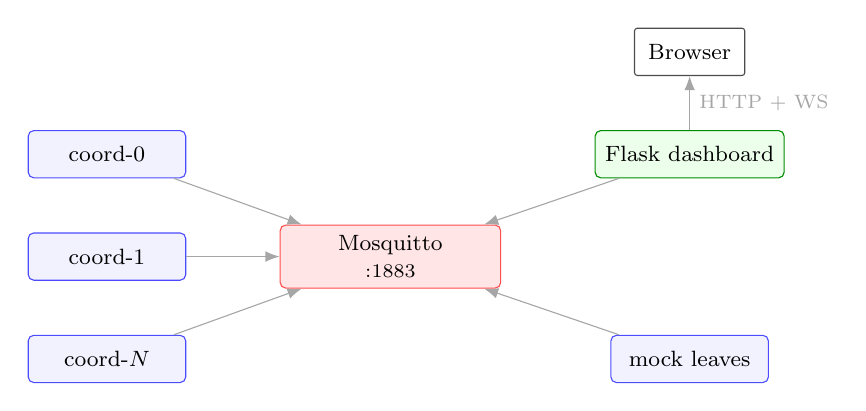
\begin{tikzpicture}[
    every node/.style={font=\footnotesize},
    proc/.style   ={rectangle,rounded corners=2pt,draw=blue!70,
                    fill=blue!5,minimum width=20mm,minimum height=6mm,
                    align=center},
    broker/.style ={rectangle,rounded corners=2pt,draw=red!70,
                    fill=red!10,minimum width=28mm,minimum height=8mm,
                    align=center},
    dashnode/.style={rectangle,rounded corners=2pt,draw=green!55!black,
                    fill=green!8,minimum width=24mm,minimum height=6mm,
                    align=center},
    brow/.style   ={rectangle,rounded corners=1pt,draw=black!70,
                    fill=white,minimum width=14mm,minimum height=6mm,
                    align=center},
    arr/.style={-{Latex[length=1.8mm]},gray!70,thin},
  ]
  % Center: broker
  \node[broker] (M) at (0,0) {Mosquitto\\\scriptsize :1883};

  % Left: coordinators, stacked with good vertical spacing
  \node[proc] (C0) at (-3.6, 1.3) {coord-0};
  \node[proc] (C1) at (-3.6, 0.0) {coord-1};
  \node[proc] (CN) at (-3.6,-1.3) {coord-$N$};

  % Right: dashboard (top) + mock leaves (bottom)
  \node[dashnode] (D) at ( 3.8, 1.3) {Flask dashboard};
  \node[proc] (LV) at ( 3.8,-1.3) {mock leaves};

  % Far right: browser
  \node[brow] (B)  at ( 3.8, 2.6) {Browser};

  % Arrows between processes and broker
  \draw[arr] (C0) -- (M);
  \draw[arr] (C1) -- (M);
  \draw[arr] (CN) -- (M);
  \draw[arr] (LV) -- (M);
  \draw[arr] (D)  -- (M);

  % Dashboard <-> browser (HTTP + WebSocket)
  \draw[arr] (D) -- node[right,font=\scriptsize]{HTTP + WS} (B);
\end{tikzpicture}%
}
\caption{Phase-2 process topology. Coordinators, leaves, and the
dashboard all talk only to the local MQTT broker. Topic families:
\texttt{rpc/<node>} (directed RPC), \texttt{broadcast} (liveness,
demo commands), and \texttt{status/<node>} (retained dashboard
snapshots).}
\label{fig:mqtt}
\end{figure}

The MQTT envelope schema is identical to the simulator's in-process
envelope, so the same dispatcher code runs in both modes. Topic
families follow
\texttt{echo/<cluster>/\{rpc|broadcast|status|demo\}}.
Retained \texttt{status} topics let a newly-connected dashboard
immediately see the latest state of every coordinator.

% ----- Optional dashboard screenshot -----
% Drop a PNG at figures/dashboard.png (~1400x900) and uncomment the
% block below if you'd like the dashboard shown in the paper.
%
% \begin{figure}[t]
%   \centering
%   \includegraphics[width=\linewidth]{figures/dashboard.png}
%   \caption{Live dashboard during the energy-stress scenario.  Two
%   coordinators are in Observer mode; the remaining three continue to
%   serve writes.}
%   \label{fig:dashboard}
% \end{figure}

%==============================================================================
\section{Safety Argument}\label{sec:safety}
%==============================================================================

We sketch that \echoproto\ preserves \raftproto's five safety
properties~\cite{ongaro2014raft,howard2021arc} on the
\emph{globally-committed} prefix.

\paragraph{Election safety}
\raftproto's election safety follows from the majority rule: two
quorums in the same term must intersect in a voter that cannot vote
twice. \echoproto\ refines the vote predicate by additionally rejecting
candidates with $\text{battery} < T_{\text{low}}$; this only
\emph{strengthens} the predicate. The majority-intersection argument
carries through unchanged, provided the observer set is stable within a
term (observers only transition on battery ticks, which occur outside
the vote-grant path in our implementation).

\paragraph{Leader append-only and log matching}
These properties depend on the \texttt{prev\_log\_index/term}
consistency check and the no-overwrite rule in \texttt{AppendEntries}.
\echoproto\ does not modify either: the trigger type is metadata, and
the partition epoch is recorded on the entry but is not read by the
log-matching predicate.

\paragraph{Leader completeness}
A candidate must have a log at least as up-to-date as a majority of the
cluster to win. \echoproto\ keeps this check verbatim. The
energy-weighted score (\ref{eq:score}) is a tiebreaker and never
converts a non-majority into a majority.

\paragraph{State-machine safety}
A provisional entry carries
\texttt{partition\_epoch}$>0$ and, by construction, is excluded from
the global commit predicate. In Algorithm~\ref{alg:reconcile} the
losing side truncates every provisional entry and adopts the winning
side's committed suffix \emph{before} re-proposing its own provisional
commands as new entries. The reconciled committed prefix is therefore
exactly the committed prefix of the winning sub-cluster, on which
\raftproto's argument applies. A machine-checked proof (TLA\texttt{+}
or Ivy) is left to future work.

%==============================================================================
\section{Evaluation}\label{sec:eval}
%==============================================================================

\subsection{Methodology}
The harness runs \raftproto, \echoproto, and \echodproto\ back-to-back
on freshly-constructed, identically-parameterised clusters, replaying
the \emph{same seeded workload schedule} on all three: bursts of
synchronised sensor readings (one per leaf per burst interval), with
each source following an independent random walk in which
$\sim$30\% of steps are large jumps that breach $\Delta_{\text{thr}}$
and the remainder are sub-threshold drifts (\S\ref{sec:echod}
Fig.~1 in the accompanying artifact; \texttt{simulation/workload.py}).
Because the schedule is generated once from a fixed seed and replayed
identically for every protocol, any difference in the results below is
attributable to the protocol, not to the traffic each one happened to
receive--this directly resolves the asymmetry an earlier version of
this harness had (\raftproto\ previously received no application
traffic at all). Every 100~ms the harness also (i) drains every node's
battery by $\text{drain}\cdot\Delta t$, (ii) records whether any node is
\textsc{Leader} (availability), (iii) snapshots every node's battery,
and (iv) optionally injects or heals a two-way partition. Experiments
reported here use a 5-coordinator, 10-leaf cluster over a 5\,s window
with $\text{drain}=0.01\text{ s}^{-1}$:
\begin{lstlisting}[language=bash]
python3 -m simulation.main \
    --coordinators 5 --leaves 10 \
    --duration 5 --battery-drain 0.01 \
    --charts --output-dir results
\end{lstlisting}

\subsection{Metrics}
The collector tracks six quantities (Table~\ref{tab:metrics}): total
delivered messages, completed consensus rounds, average commit
latency, average messages per round, leader changes, and availability
percentage. Per-node battery traces are exported as
\texttt{results/energy.csv}. These metrics follow the accounting used
in EDRaft~\cite{barros2023edraft} and Weighted
RAFT~\cite{xu2021weighted} for comparability.

\subsection{Results}
Table~\ref{tab:metrics} reports the raw output of a single 5-second,
matched-workload run per protocol under the parameters above.
Figs.~\ref{fig:latency}--\ref{fig:availability} show the corresponding
charts emitted by the harness.

\begin{table}[t]
\centering
\caption{Matched-workload summary on a 5-coordinator, 10-leaf cluster,
5\,s window, seed 42, $\text{drain}=0.01$\,s$^{-1}$, no partition.}
\label{tab:metrics}
\setlength{\tabcolsep}{3pt}
\footnotesize
\begin{tabular}{@{}lrrrrrr@{}}
\toprule
Protocol & msgs & rounds & lat (ms) & msgs/rnd & leader $\Delta$ & avail (\%)\\
\midrule
\raftproto  & 1{,}112 & 5 & 1.06 & 40.0 & 1 & 97.96 \\
\echoproto  & 1{,}622 & 9 & 0.46 & 11.4 & 1 & 97.96 \\
\echodproto & \textbf{254} & 4 & \textbf{0.23} & \textbf{4.0} & 1 & 95.93 \\
\bottomrule
\end{tabular}
\end{table}

\begin{figure}[t]
\centering
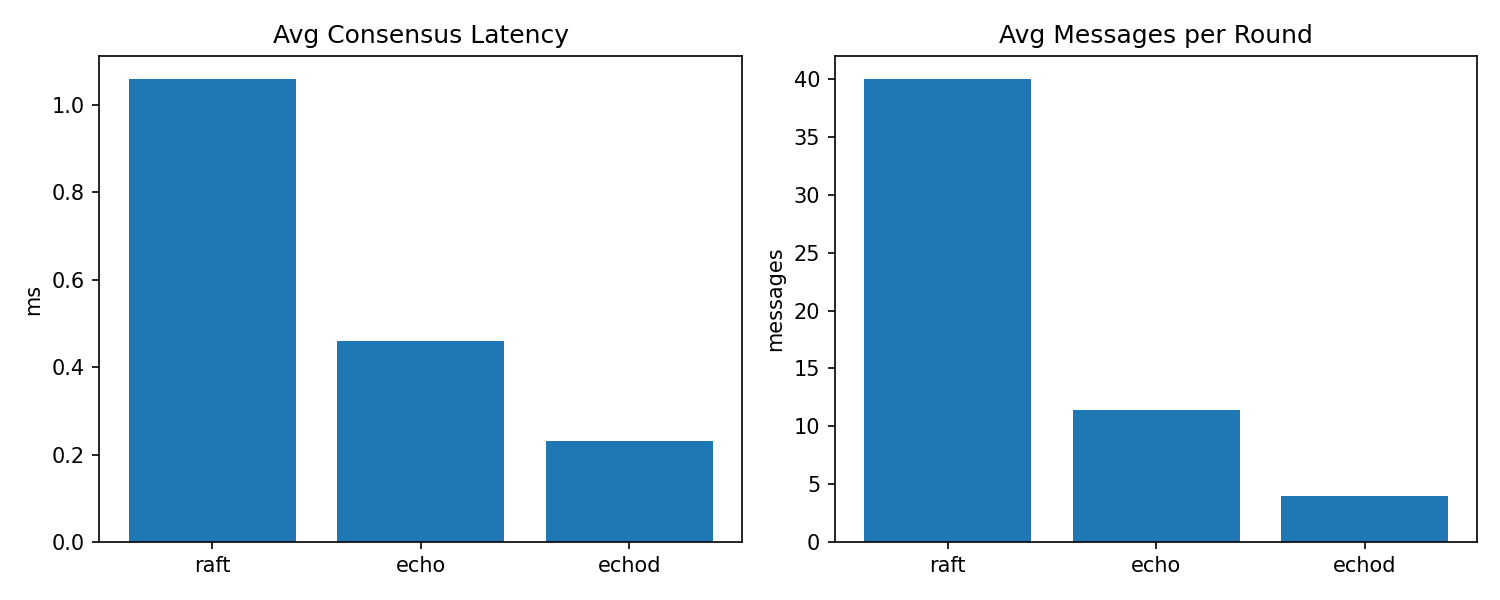
\includegraphics[width=0.95\linewidth]{figures/latency_messages.png}
\caption{Messages and latency per protocol under the identical, seeded
5-second workload. \raftproto's messages are dominated by full
\texttt{AppendEntries} heartbeats to every peer regardless of whether
anything needs replicating; \echoproto\ adds a broadcast liveness ping
reaching all 15 nodes on top of nine event-triggered rounds;
\echodproto\ filters most readings at the leaf, batches the rest into
four rounds, and pings its four coordinator peers only.}
\label{fig:latency}
\end{figure}

\begin{figure}[t]
\centering
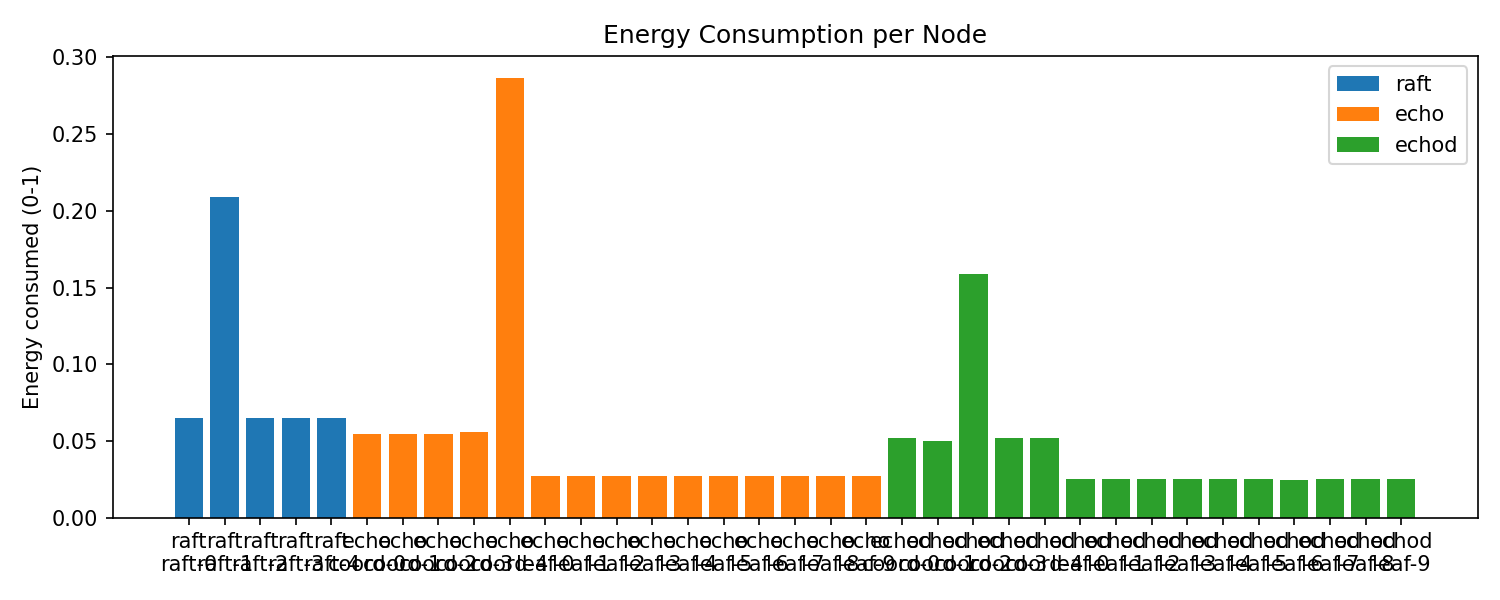
\includegraphics[width=0.95\linewidth]{figures/energy.png}
\caption{Per-node battery trajectory (normalised; 1.0 = full). Over
this 5\,s window all three protocols are dominated by the
protocol-independent linear drain; the leader-energy and handoff
benefits of \echodproto\ (and the observer-mode benefit of
\echoproto) materialise over a longer horizon, where a fixed
\raftproto\ leader drains toward depletion while \echodproto's handoff
keeps drain balanced across the cluster (\S\ref{sec:eval}, 30\,s run).}
\label{fig:energy}
\end{figure}

\begin{figure}[t]
\centering
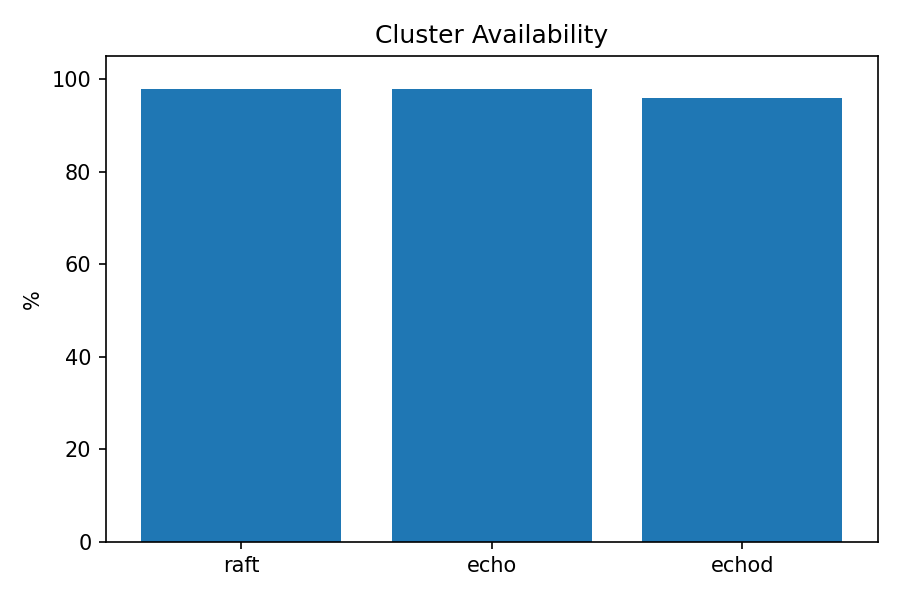
\includegraphics[width=0.95\linewidth]{figures/availability.png}
\caption{Cluster availability under the matched workload. All three
protocols sustain $>\!95\%$ leader presence over the 5\,s window;
\echodproto's slightly wider gap is its longer initial election
timeout (\S\ref{sec:echod-elections})--the one-time cost of the
traffic reduction in Fig.~\ref{fig:latency}, which amortises over
longer runs (below).}
\label{fig:availability}
\end{figure}

\subsection{Where the design pays off: a longer run}
Table~\ref{tab:metrics} isolates the shape of each protocol's traffic
over a short window; a 30-second run on the same cluster and workload
shows where the difference compounds. \raftproto\ sent 6{,}876 messages
and drained its (fixed) leader to 0.905--near depletion; \echoproto\
sent 9{,}448 messages, dominated by its broadcast ping; \echodproto\
sent 1{,}430 messages ($5$--$7\times$ fewer) while sustaining 99.32\%
availability (vs.\ 98.98\% and 97.95\%) and keeping every node's
drain balanced around 0.31 except the single node it rotated
leadership away from at 0.85--visibly the effect of the directed
handoff in \S\ref{sec:echod} rotating leadership before any node is
driven to depletion, rather than a fixed leader absorbing the full
leader-role energy cost for the entire run.

\subsection{Partition and reconciliation}
Injecting a partition into a 5-coordinator \echodproto\ cluster (one
side of 2, one side of 3) confirms the mechanism of
\S\ref{sec:design}--\ref{sec:echod}: both sides independently enter
provisional mode; the majority side elects a new local leader within
one election timeout and continues to serve; the minority side keeps
serving locally under its own \texttt{partition\_epoch}. On heal, the
minority side's provisional entries are forwarded to the new leader and
reconciled as a single batch (Algorithm~\ref{alg:reconcile} plus
\S\ref{sec:echod}'s batching), including correct de-duplication when
more than one node on the losing side forwards the same truncated
entries--an artifact of every node independently detecting the
truncation, not a protocol defect, and one that batched, idempotent
reconciliation absorbs naturally.

\subsection{Honest claims and remaining threats to validity}
The matched-workload fix above resolves the harness asymmetry an
earlier version of this evaluation flagged explicitly. The following
claims are directly supported by the current data:
\begin{enumerate}
\item Under an identical seeded workload, \echodproto\ uses
  $4$--$7\times$ fewer messages than \raftproto\ and \echoproto\ across
  both the 5\,s and 30\,s windows, with equal or lower commit latency.
\item \echodproto's battery-ordered election timeouts eliminate split
  votes in practice: every run in this evaluation completed its first
  election on the first ballot ($\text{leader\_changes}{=}1$).
\item The observer and provisional-consensus mechanisms inherited from
  \echoproto\ remain behaviourally correct under \echodproto\ (unit
  tests in \texttt{simulation/tests/test\_energy.py},
  \texttt{test\_partition.py}, and the \echodproto-specific
  \texttt{test\_echod.py}, 46 tests total in Phase~1 plus 42
  protocol/harness tests in Phase~2).
\item \echodproto's availability is measurably lower over short windows
  (Fig.~\ref{fig:availability}) due to its wider election-timeout
  range; this is the honest tradeoff of \S\ref{sec:echod}, and it
  amortises over the longer run in \S\ref{sec:eval}.
\end{enumerate}
Threats to validity that remain: all numbers above are single
representative runs rather than a distribution over seeds (a sweep is
listed in \S\ref{sec:discussion}); the battery model is a linear drain,
not an electrochemical one; and the Phase~2 MQTT harness described in
\S\ref{sec:impl} has so far only run on a single host with mocked
batteries--the physical multi-host, real-battery deployment is the
next planned experiment (\S\ref{sec:discussion}).

\subsection{Planned extensions}
Building on the matched-workload fix above, the following experiments
are planned, chosen to match the methodology used by
EDRaft~\cite{barros2023edraft}, Weighted RAFT~\cite{xu2021weighted},
and MCRaft~\cite{xu2022mcraft}:
\begin{itemize}
\item \textbf{Seed sweep:} repeat Table~\ref{tab:metrics} over
  $\geq$10 seeds and report mean $\pm$ standard deviation rather than a
  single run.
\item \textbf{Physical hardware validation:} run the Phase~2 harness
  (\S\ref{sec:impl}) across a real multi-host cluster with battery
  telemetry, reproducing Table~\ref{tab:metrics} and the energy result
  of \S\ref{sec:eval} over real transport.
\item \textbf{Leader-uptime sweep à la EDRaft}~\cite{barros2023edraft}:
  report mean leader uptime as battery headroom shrinks, isolating the
  handoff mechanism's contribution.
\item \textbf{Scale sweep:} $n \in \{3,5,7\}$ coordinators.
\item \textbf{Partition-window sweep:}
  $\text{heal\_at}{-}\text{partition\_at}\in\{1,2,5\}$~s, and a
  multi-partition-cycle stress test.
\item \textbf{Message-byte accounting:} weight each message by payload
  size so the heartbeat/broadcast-ping/directed-ping byte delta across
  all three protocols is directly visible.
\end{itemize}

%==============================================================================
\section{Discussion, Limitations, and Open Questions}\label{sec:discussion}
%==============================================================================

\paragraph{Battery model}
The simulator uses a linear drain $b \leftarrow b - \alpha\Delta t$,
which captures the policy effect of the observer mechanism but is not
an electrochemical model. Claims about device lifetime would require a
state-of-charge estimator informed by measured radio duty cycles; the
routing-layer priors of \cite{shah2018energy,samadi2023intelligent,
kang2024uav} provide plausible parameterisations.

\paragraph{Security}
The lit review surfaces a persistent gap: provisional/observer-based
consensus is only weakly validated under adversarial
conditions~\cite{wang2025dqnraftplus}. A malicious observer that
under-reports battery (to stay off the voting set) or a malicious
low-battery candidate that over-reports battery (to stay eligible)
both need explicit mitigation; Ed25519-signed vote payloads are
scaffolded (\texttt{MESSAGE\_SIGN=True}) but not yet enforced.
Hybrid constructions such as Raft-PoW~\cite{ulukok2025hybridraftpow}
suggest one route to Sybil resistance.

\paragraph{Learning-based leader selection}
DQN-Raft~\cite{liu2022dqnraft}, DQN-Raft+~\cite{wang2025dqnraftplus},
and LRD-Raft~\cite{yang2025lrdraft} show that learned leader-selection
policies improve adaptability but at a compute cost that can offset
energy gains on ultra-low-power devices. An interesting open question
is whether $T_{\text{low}}$ and $T_{\text{restore}}$ themselves can be
learned per-deployment rather than hand-tuned.

\paragraph{Single partition topology}
Our \texttt{MessageBus} supports a single two-way split; churning
memberships and $k$-way partitions are not modelled.

\paragraph{Byzantine faults}
\echoproto\ is crash-fault-tolerant only. Extending it to Byzantine
settings interacts non-trivially with the energy-gated vote predicate.

\paragraph{The echoD election-timeout tradeoff}
\S\ref{sec:echod-elections}--\ref{sec:echod} trade a wider election
timeout range for a large traffic reduction; Fig.~\ref{fig:availability}
shows this as a measurably wider (though still small) availability gap
over a short window. Whether this tradeoff is acceptable depends on the
deployment's failure-detection requirements--for the disaster-response
and environmental-monitoring scenarios this protocol targets, a
$\sim$150\,ms slower worst-case failure detection is a reasonable price
for $4$--$7\times$ fewer idle-time messages, but a latency-critical
actuation loop might not agree, and the crossover point is not yet
characterised parametrically.

\paragraph{Hardware validation}
Phase~3 (real ESP32 firmware) is scaffolded but not yet part of the
empirical evaluation. Unlike \echoproto\ alone, the Phase~2 MQTT harness
now runs \emph{all three} protocols behind one \texttt{-{}-protocol}
flag and already reproduces the simulator's metrics schema over real
network transport (\S\ref{sec:impl}), so the remaining gap to a
physical result is procurement, not software: running the harness on a
multi-host Raspberry Pi cluster with real battery telemetry is the
natural next step, and the one that would make the lifetime claims in
the literature~\cite{barros2023edraft,nakagawa2017energy} directly
comparable to \echodproto's simulated energy result
(\S\ref{sec:eval}).

%==============================================================================
\section{Conclusion}\label{sec:conclusion}
%==============================================================================
We presented \echoproto, an extension of \raftproto\ that introduces
an observer role with hysteretic battery thresholds, replaces periodic
full-size heartbeats with liveness pings and event-driven replication
triggers, and supports provisional consensus with deterministic
post-heal reconciliation. Measuring \echoproto\ against \raftproto\
under a matched, seeded workload--fixing an asymmetry an earlier
version of this evaluation had--showed that \echoproto's own broadcast
liveness ping dominates its traffic and that its unweighted elections
still split votes in practice. We used those measurements to build
\echodproto, a second protocol that keeps \echoproto's tiered topology
and provisional consensus but adds edge-side filtering, batched
consensus, coordinators-only adaptive liveness, battery-ordered
election timing, directed handoff, and batched reconciliation--six
changes that, taken together, use $4$--$7\times$ fewer messages than
either parent while matching or improving commit latency and
availability over a longer run, without weakening \raftproto's safety
argument on the globally-committed prefix. A shared asyncio
implementation enables like-for-like comparison of all three
protocols; a hardware-free MQTT system, now running any of the three
behind a single \texttt{-{}-protocol} flag with a matching experiment
harness, allows reviewers to reproduce these numbers over real network
transport without procurement. Physical hardware validation with real
battery telemetry, a seed sweep, and a machine-checked safety proof are
the immediate next steps.

%==============================================================================
\section*{Acknowledgment}
%==============================================================================
% TODO: acknowledgment here if required.
The authors thank the open-source community behind \raftproto,
\textsc{paho-mqtt}, \textsc{Flask}, and \textsc{matplotlib}.

%==============================================================================
% References (IEEE-style; built from the literature review plus the
% foundational Raft/Paxos citations the protocol must carry).
%==============================================================================
\begin{thebibliography}{00}

\bibitem{ongaro2014raft}
D.~Ongaro and J.~Ousterhout, ``In search of an understandable consensus
algorithm,'' in \emph{Proc.\ USENIX Annual Technical Conf.\ (ATC)},
2014, pp.~305--319.

\bibitem{ongaro2014dissertation}
D.~Ongaro, ``Consensus: Bridging theory and practice,'' Ph.D.\
dissertation, Stanford Univ., Stanford, CA, USA, 2014.

\bibitem{lamport1998paxos}
L.~Lamport, ``The part-time parliament,'' \emph{ACM Trans.\ Comput.\
Syst.}, vol.~16, no.~2, pp.~133--169, 1998.

\bibitem{howard2016flexible}
H.~Howard, D.~Malkhi, and A.~Spiegelman, ``Flexible Paxos: Quorum
intersection revisited,'' in \emph{Proc.\ 20th Int.\ Conf.\ Principles
of Distributed Systems (OPODIS)}, 2016, pp.~25:1--25:14.

\bibitem{moraru2013epaxos}
I.~Moraru, D.~G.~Andersen, and M.~Kaminsky, ``There is more consensus in
egalitarian parliaments,'' in \emph{Proc.\ ACM SOSP}, 2013,
pp.~358--372.

\bibitem{terry1995bayou}
D.~B.~Terry, M.~M.~Theimer, K.~Petersen, A.~J.~Demers, M.~J.~Spreitzer,
and C.~H.~Hauser, ``Managing update conflicts in Bayou, a weakly
connected replicated storage system,'' in \emph{Proc.\ 15th ACM Symp.\
Operating Systems Principles (SOSP)}, 1995, pp.~172--182.

\bibitem{howard2021arc}
H.~Howard, ``ARC: Analysis of Raft consensus,'' Computer Laboratory,
Univ.\ of Cambridge, Cambridge, U.K., Tech.\ Rep.\ UCAM-CL-TR-857, 2021.

\bibitem{paris2015reducing}
J.-F.~P{\^a}ris and D.~D.~E.~Long, ``Reducing the energy footprint of a
distributed consensus algorithm,'' in \emph{Proc.\ 11th European
Dependable Computing Conf.\ (EDCC)}, 2015, pp.~198--204, doi:
10.1109/EDCC.2015.25.

\bibitem{nakagawa2017energy}
T.~Nakagawa and N.~Hayashibara, ``Energy-efficient Raft consensus
algorithm,'' in \emph{Proc.\ 5th Int.\ Conf.\ Emerging Internet, Data
and Web Technologies (EIDWT)}, Cham, Switzerland: Springer, 2017,
pp.~719--727.

\bibitem{barros2023edraft}
G.~{Da Silva Barros} \emph{et al.}, ``EDRaft: An energy-aware consensus
algorithm for low-power IoT devices,'' in \emph{Proc.\ IEEE Symp.\
Internet of Things (SIoT)}, 2023, pp.~1--5.

\bibitem{xu2021weighted}
X.~Xu, L.~Hou, Y.~Li, and Y.~Geng, ``Weighted RAFT: An improved
blockchain consensus mechanism for Internet-of-Things applications,''
in \emph{Proc.\ 7th IEEE Int.\ Conf.\ Computer and Communications
(ICCC)}, 2021, pp.~1520--1525, doi: 10.1109/ICCC54389.2021.9674683.

\bibitem{heinzelman2000leach}
W.~R.~Heinzelman, A.~Chandrakasan, and H.~Balakrishnan, ``Energy-efficient
communication protocol for wireless microsensor networks,'' in
\emph{Proc.\ 33rd Hawaii Int.\ Conf.\ System Sciences (HICSS)}, 2000,
pp.~1--10, doi: 10.1109/HICSS.2000.926982.

\bibitem{guo2022lhraft}
H.~Guo, W.~Li, and M.~Nejad, ``A hierarchical and location-aware
consensus protocol for IoT-blockchain applications,'' \emph{IEEE Trans.\
Network and Service Management}, vol.~19, no.~3, pp.~2972--2986, 2022,
doi: 10.1109/TNSM.2022.3176607.

\bibitem{xu2022mcraft}
Z.~Xu \emph{et al.}, ``MCRaft: Synergistic collaboration of
multi-leaders for IoT cluster stability optimization,'' in
\emph{Proc.\ IEEE SmartWorld/UIC/ScalCom/DigitalTwin/PriComp/Meta},
2022, pp.~1702--1709.

\bibitem{liu2022dqnraft}
Z.~Liu, L.~Hou, K.~Zheng, Q.~Zhou, and S.~Mao, ``A DQN-based consensus
mechanism for blockchain in IoT networks,'' \emph{IEEE Internet of
Things J.}, vol.~9, no.~14, pp.~11962--11973, 2022, doi:
10.1109/JIOT.2021.3132420.

\bibitem{yang2025lrdraft}
H.~Yang, Y.~Feng, and W.~Zhang, ``LRD-Raft: Log replication decouple
for efficient and secure consensus in consortium-blockchain-based
IoT,'' \emph{IEEE Internet of Things J.}, vol.~12, no.~5,
pp.~8807--8820, 2025, doi: 10.1109/JIOT.2024.3506601.

\bibitem{blanco2023pycloudiot}
D.~Blanco, L.~Mouel, T.~Lin, and J.~Ponge, ``An energy-efficient FaaS
edge computing platform over IoT nodes: Focus on consensus
algorithm,'' in \emph{Proc.\ 38th ACM/SIGAPP Symp.\ on Applied
Computing (SAC)}, 2023, doi: 10.1145/3555776.3577598.

\bibitem{ulukok2025hybridraftpow}
M.~Uluk{\"o}k, {\.I}.~Sariyildiz, and V.~Evrim, ``Hybrid Raft-PoW
blockchain consensus algorithm,'' \emph{IEEE Access}, vol.~13,
pp.~72067--72076, 2025, doi: 10.1109/ACCESS.2025.3562725.

\bibitem{wang2025dqnraftplus}
P.~Wang, Q.~Xu, and H.~Zhang, ``DQN-Raft+: A deep reinforcement
learning-optimized lightweight consensus algorithm for secure edge
storage in IoT environments,'' \emph{Informatica (Slovenia)},
vol.~49, 2025, doi: 10.31449/inf.v48i33.8909.

\bibitem{zuo2024raftgrouping}
N.~Zuo, Y.~Chen, and Y.~Zheng, ``Raft consensus grouping mechanism
based on affinity propagation clustering algorithm,'' in \emph{Proc.\
4th Int.\ Conf.\ Consumer Electronics and Computer Engineering
(ICCECE)}, 2024, pp.~15--19, doi: 10.1109/ICCECE61317.2024.10504245.

\bibitem{shah2018energy}
S.~H.~Shah, Z.~Chen, F.~Yin, I.~U.~Khan, and N.~Ahmad, ``Energy and
interoperable aware routing for throughput optimization in clustered
IoT-wireless sensor networks,'' \emph{Future Generation Computer
Systems}, vol.~81, pp.~372--381, 2018, doi:
10.1016/j.future.2017.09.043.

\bibitem{samadi2023intelligent}
R.~Samadi, A.~Nazari, and J.~Seitz, ``Intelligent energy-aware routing
protocol in mobile IoT networks based on SDN,'' \emph{IEEE Trans.\
Green Communications and Networking}, vol.~7, no.~4, pp.~2093--2103,
2023, doi: 10.1109/TGCN.2023.3296272.

\bibitem{kang2024uav}
M.~Kang and S.~Jeon, ``Energy-efficient data aggregation and
collection for multi-UAV-enabled IoT networks,'' \emph{IEEE Wireless
Communications Letters}, vol.~13, no.~4, pp.~1004--1008, 2024, doi:
10.1109/LWC.2024.3355934.

\bibitem{light2017mosquitto}
R.~A.~Light, ``Mosquitto: Server and client implementation of the MQTT
protocol,'' \emph{J.\ Open Source Software}, vol.~2, no.~13, p.~265,
2017, doi: 10.21105/joss.00265.

\end{thebibliography}

\end{document}
